\documentclass[aspectratio=169]{beamer}
\usetheme{Madrid}
\usecolortheme{whale}

\usepackage{amsmath,amssymb,amsthm}
\usepackage{tikz}
\usepackage{booktabs}

\title{Q-Learning: A Historical Synthesis}
\subtitle{Robbins-Monro + Bellman + Epsilon-Greedy}
\author{A Journey Through Reinforcement Learning History}
\date{}

\begin{document}

\begin{frame}
\titlepage
\end{frame}

\begin{frame}{Outline}
\tableofcontents
\end{frame}

%==============================================================================
\section{Part I: Robbins-Monro Stochastic Approximation (1951)}
%==============================================================================

\begin{frame}{The Problem of Root Finding Under Noise}
\textbf{Classical Problem:} Find $\theta^*$ such that $M(\theta^*) = 0$

\vspace{0.5cm}
\textbf{Challenge:} We cannot observe $M(\theta)$ directly---only noisy samples
\[
Y = M(\theta) + \varepsilon
\]
where $\varepsilon$ is random noise with $\mathbb{E}[\varepsilon] = 0$.

\vspace{0.5cm}
\textbf{Context (1951):}
\begin{itemize}
    \item Herbert Robbins \& Sutton Monro at UNC Chapel Hill
    \item Motivated by bioassay problems (finding drug dosage thresholds)
    \item Published: ``A Stochastic Approximation Method'' (Annals of Math. Stat.)
\end{itemize}
\end{frame}

\begin{frame}{The Robbins-Monro Algorithm}
\textbf{The Update Rule:}
\[
\theta_{n+1} = \theta_n - a_n Y_n
\]

where $Y_n = M(\theta_n) + \varepsilon_n$ is a noisy observation of $M(\theta_n)$.

\vspace{0.5cm}
\textbf{Key Conditions on Step Sizes:}
\[
\sum_{n=1}^{\infty} a_n = \infty \quad \text{and} \quad \sum_{n=1}^{\infty} a_n^2 < \infty
\]

\vspace{0.3cm}
\textbf{Example:} $a_n = 1/n$ satisfies both conditions.

\vspace{0.5cm}
\textbf{Theorem (Robbins-Monro 1951):} Under mild regularity conditions,
\[
\theta_n \xrightarrow{\text{a.s.}} \theta^* \quad \text{as } n \to \infty
\]
\end{frame}

\begin{frame}{Why Robbins-Monro Matters for RL}
\textbf{The Template for Learning from Noisy Feedback:}
\[
\text{New Estimate} = \text{Old Estimate} + \text{Step Size} \times \text{Error Signal}
\]

\vspace{0.5cm}
\textbf{Intuition:}
\begin{itemize}
    \item Large steps early (explore the space)
    \item Small steps later (converge precisely)
    \item Noise averages out over time
\end{itemize}

\vspace{0.5cm}
\textbf{This pattern appears everywhere in RL:}
\begin{itemize}
    \item TD-learning
    \item Q-learning
    \item Policy gradient methods
    \item Actor-critic algorithms
\end{itemize}
\end{frame}

%==============================================================================
\section{Part II: Bellman's Dynamic Programming (1957)}
%==============================================================================

\begin{frame}{Richard Bellman and the Curse of Dimensionality}
\textbf{Richard Bellman (1920--1984):}
\begin{itemize}
    \item RAND Corporation, 1950s
    \item Coined ``dynamic programming'' (1953)
    \item Published \textit{Dynamic Programming} (1957)
\end{itemize}

\vspace{0.5cm}
\textbf{The Core Insight:}

Optimal decisions have a recursive structure---the \textit{principle of optimality}.

\vspace{0.3cm}
\begin{quote}
``An optimal policy has the property that whatever the initial state and initial decision are, the remaining decisions must constitute an optimal policy with regard to the state resulting from the first decision.''
\end{quote}
\end{frame}

\begin{frame}{Deriving Bellman from Random Horizons}
\textbf{Key Insight:} Let horizon $T \sim \text{Geometric}(1-\gamma)$, so $P(T \geq 1) = \gamma$.

\vspace{0.3cm}
Define the $Q$-function as expected cumulative reward over random horizon:
\[
Q(s,a) = \mathbb{E}\left[ \sum_{k=0}^{T} r_k \;\Big|\; s_0 = s, a_0 = a \right]
\]

\textbf{Unroll one step:}
\begin{align*}
Q(s,a) &= \mathbb{E}[r_0] + P(T \geq 1) \cdot \mathbb{E}\left[ \sum_{k=1}^{T} r_k \;\Big|\; T \geq 1 \right] \\[4pt]
&= R(s,a) + \gamma \cdot \mathbb{E}_{s' \sim P(\cdot|s,a)}\left[ \max_{a'} Q(s', a') \right]
\end{align*}

\vspace{0.2cm}
The memoryless property of the geometric distribution gives recursion!
\end{frame}

\begin{frame}{The Bellman Equation}
\textbf{Value Function:} $V^*(s)$ = optimal expected cumulative reward from state $s$

\vspace{0.3cm}
\textbf{Bellman Optimality Equation:}
\[
V^*(s) = \max_a \left[ R(s,a) + \gamma \sum_{s'} P(s'|s,a) V^*(s') \right]
\]

\vspace{0.5cm}
\textbf{Action-Value Form} (crucial for Q-learning):
\[
Q^*(s,a) = R(s,a) + \gamma \sum_{s'} P(s'|s,a) \max_{a'} Q^*(s',a')
\]

\vspace{0.5cm}
\textbf{The $Q$-function:} Expected return starting from state $s$, taking action $a$, then acting optimally.
\end{frame}

\begin{frame}{The Contraction Property}
\textbf{Bellman Operator:}
\[
(TQ)(s,a) = R(s,a) + \gamma \sum_{s'} P(s'|s,a) \max_{a'} Q(s',a')
\]

\vspace{0.5cm}
\textbf{Key Property:} $T$ is a contraction in the max-norm:
\[
\|TQ_1 - TQ_2\|_\infty \leq \gamma \|Q_1 - Q_2\|_\infty
\]

\vspace{0.5cm}
\textbf{Consequence (Banach Fixed Point Theorem):}
\begin{itemize}
    \item $Q^*$ exists and is unique
    \item Repeated application $Q \leftarrow TQ$ converges to $Q^*$
    \item This is \textbf{value iteration}
\end{itemize}

\vspace{0.3cm}
\textbf{Problem:} Requires knowing $P(s'|s,a)$ and $R(s,a)$---the model!
\end{frame}

%==============================================================================
\section{Part III: Exploration vs.\ Exploitation}
%==============================================================================

\begin{frame}{The Exploration-Exploitation Dilemma}
\textbf{The Fundamental Tradeoff:}
\begin{itemize}
    \item \textbf{Exploitation:} Use current knowledge to maximize reward
    \item \textbf{Exploration:} Gather new information for future benefit
\end{itemize}

\vspace{0.5cm}
\textbf{Historical Roots:}
\begin{itemize}
    \item Sequential experimental design (1940s--1950s)
    \item Multi-armed bandit problem (Robbins 1952)
    \item Thompson Sampling (Thompson 1933, rediscovered later)
\end{itemize}

\vspace{0.5cm}
\textbf{Why It Matters:}

A purely greedy learner may get stuck in local optima, never discovering better actions.
\end{frame}

\begin{frame}{Epsilon-Greedy: Simple and Effective}
\textbf{The Algorithm:}
\[
a = \begin{cases}
\arg\max_a Q(s,a) & \text{with probability } 1-\varepsilon \\
\text{random action} & \text{with probability } \varepsilon
\end{cases}
\]

\vspace{0.5cm}
\textbf{Properties:}
\begin{itemize}
    \item Ensures every action tried infinitely often (given infinite time)
    \item Simple to implement and analyze
    \item $\varepsilon$ can decay over time: $\varepsilon_t \to 0$
\end{itemize}

\vspace{0.5cm}
\textbf{Historical Note:}
\begin{itemize}
    \item No single ``inventor''---emerged from operations research
    \item Closely related to randomized strategies in game theory
    \item Became standard in RL through Sutton \& Barto's work (1980s)
\end{itemize}
\end{frame}

\begin{frame}{Why Exploration is Necessary for Convergence}
\textbf{For Q-learning to converge, we need:}

\vspace{0.3cm}
Every state-action pair $(s,a)$ must be visited infinitely often.

\vspace{0.5cm}
\textbf{Epsilon-greedy guarantees this:}
\begin{itemize}
    \item Probability of any action in any state $\geq \varepsilon / |A|$
    \item Under mild reachability assumptions, all $(s,a)$ pairs visited
\end{itemize}

\vspace{0.5cm}
\textbf{Alternatives:}
\begin{itemize}
    \item Boltzmann/softmax exploration
    \item Upper Confidence Bound (UCB)
    \item Optimism in the face of uncertainty
    \item Intrinsic motivation / curiosity
\end{itemize}
\end{frame}

%==============================================================================
\section{Part IV: The Synthesis---Q-Learning (1989)}
%==============================================================================

\begin{frame}{Christopher Watkins and Q-Learning}
\textbf{Chris Watkins (1989):}
\begin{itemize}
    \item PhD thesis: ``Learning from Delayed Rewards'' (Cambridge)
    \item Published with Dayan (1992): convergence proof
\end{itemize}

\vspace{0.5cm}
\textbf{The Breakthrough:}

Combine Bellman's equation with Robbins-Monro updates to learn $Q^*$ \textbf{without knowing the model}.

\vspace{0.5cm}
\textbf{The Q-Learning Update:}
\[
Q(s_t, a_t) \leftarrow Q(s_t, a_t) + \alpha_t \left[ r_t + \gamma \max_{a'} Q(s_{t+1}, a') - Q(s_t, a_t) \right]
\]

\vspace{0.3cm}
This is Robbins-Monro applied to the Bellman equation!
\end{frame}

\begin{frame}{Dissecting the Q-Learning Update}
\[
Q(s_t, a_t) \leftarrow Q(s_t, a_t) + \alpha_t \underbrace{\left[ r_t + \gamma \max_{a'} Q(s_{t+1}, a') - Q(s_t, a_t) \right]}_{\text{Temporal Difference (TD) Error}}
\]

\vspace{0.5cm}
\begin{tabular}{ll}
\toprule
\textbf{Component} & \textbf{Origin} \\
\midrule
$\alpha_t$ (step size) & Robbins-Monro (1951) \\
$r_t + \gamma \max_{a'} Q(s_{t+1}, a')$ & Bellman target (1957) \\
TD error structure & Stochastic approximation \\
Exploration policy & Epsilon-greedy / bandits \\
\bottomrule
\end{tabular}

\vspace{0.5cm}
\textbf{Key insight:} The observed $(r_t, s_{t+1})$ is a \textit{sample} from the unknown MDP dynamics.
\end{frame}

\begin{frame}{The Convergence Theorem}
\textbf{Theorem (Watkins \& Dayan, 1992):}

Q-learning converges to $Q^*$ with probability 1, provided:

\vspace{0.3cm}
\begin{enumerate}
    \item All state-action pairs visited infinitely often
    \item Step sizes satisfy: $\sum_t \alpha_t = \infty$ and $\sum_t \alpha_t^2 < \infty$
    \item Rewards are bounded
\end{enumerate}

\vspace{0.5cm}
\textbf{Proof Sketch:}
\begin{itemize}
    \item View Q-learning as stochastic approximation (Robbins-Monro)
    \item The Bellman operator is a contraction
    \item Apply general SA convergence theory (e.g., Jaakkola et al.\ 1994)
\end{itemize}

\vspace{0.3cm}
\textbf{Epsilon-greedy ensures condition 1!}
\end{frame}

\begin{frame}{The Complete Q-Learning Algorithm}
\begin{enumerate}
    \item Initialize $Q(s,a)$ arbitrarily for all $(s,a)$
    \item For each episode:
    \begin{enumerate}
        \item Initialize state $s$
        \item For each step:
        \begin{itemize}
            \item Choose $a$ from $s$ using $\varepsilon$-greedy w.r.t.\ $Q$
            \item Take action $a$, observe $r$, $s'$
            \item Update:
            \[
            Q(s,a) \leftarrow Q(s,a) + \alpha \left[ r + \gamma \max_{a'} Q(s',a') - Q(s,a) \right]
            \]
            \item $s \leftarrow s'$
        \end{itemize}
        \item Until $s$ is terminal
    \end{enumerate}
\end{enumerate}

\vspace{0.3cm}
\textbf{Three pillars working together:}
\begin{itemize}
    \item Bellman equation provides the learning target
    \item Robbins-Monro provides the update mechanism
    \item Epsilon-greedy provides the exploration
\end{itemize}
\end{frame}

%==============================================================================
\section{Part V: Historical Timeline and Legacy}
%==============================================================================

\begin{frame}{Timeline: The Road to Q-Learning}
\begin{center}
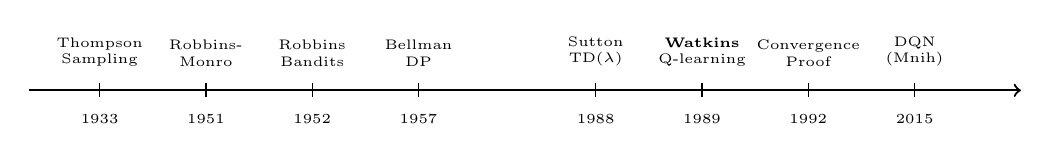
\begin{tikzpicture}[scale=0.9]
\draw[thick,->] (0,0) -- (14,0);

% Tick marks and labels
\foreach \x/\year in {1/1933, 2.5/1951, 4/1952, 5.5/1957, 8/1988, 9.5/1989, 11/1992, 12.5/2015} {
    \draw (\x,0.1) -- (\x,-0.1);
}

\node[below,font=\tiny] at (1,-0.2) {1933};
\node[above,font=\tiny,text width=1.5cm,align=center] at (1,0.2) {Thompson\\Sampling};

\node[below,font=\tiny] at (2.5,-0.2) {1951};
\node[above,font=\tiny,text width=1.5cm,align=center] at (2.5,0.2) {Robbins-\\Monro};

\node[below,font=\tiny] at (4,-0.2) {1952};
\node[above,font=\tiny,text width=1.5cm,align=center] at (4,0.2) {Robbins\\Bandits};

\node[below,font=\tiny] at (5.5,-0.2) {1957};
\node[above,font=\tiny,text width=1.5cm,align=center] at (5.5,0.2) {Bellman\\DP};

\node[below,font=\tiny] at (8,-0.2) {1988};
\node[above,font=\tiny,text width=1.5cm,align=center] at (8,0.2) {Sutton\\TD($\lambda$)};

\node[below,font=\tiny] at (9.5,-0.2) {1989};
\node[above,font=\tiny,text width=1.5cm,align=center] at (9.5,0.2) {\textbf{Watkins}\\Q-learning};

\node[below,font=\tiny] at (11,-0.2) {1992};
\node[above,font=\tiny,text width=1.5cm,align=center] at (11,0.2) {Convergence\\Proof};

\node[below,font=\tiny] at (12.5,-0.2) {2015};
\node[above,font=\tiny,text width=1.5cm,align=center] at (12.5,0.2) {DQN\\(Mnih)};
\end{tikzpicture}
\end{center}

\vspace{0.5cm}
\textbf{Key Contributors:}
\begin{itemize}
    \item Robbins \& Monro: Stochastic approximation framework
    \item Bellman: Optimality principle and recursive structure
    \item Sutton: Temporal difference learning bridge
    \item Watkins: The synthesis into Q-learning
\end{itemize}
\end{frame}

\begin{frame}{The Legacy: From Q-Learning to Deep RL}
\textbf{The Original Formula Lives On:}
\[
Q(s,a) \leftarrow Q(s,a) + \alpha \left[ r + \gamma \max_{a'} Q(s',a') - Q(s,a) \right]
\]

\vspace{0.3cm}
\textbf{Modern Extensions:}
\begin{itemize}
    \item \textbf{DQN (2015):} $Q$ represented by deep neural network
    \item \textbf{Double DQN:} Reduces overestimation bias
    \item \textbf{Dueling DQN:} Separates value and advantage
    \item \textbf{Rainbow:} Combines multiple improvements
    \item \textbf{Distributional RL:} Learn full return distribution
\end{itemize}

\vspace{0.5cm}
\textbf{The three pillars remain:}

Bellman structure $+$ stochastic approximation $+$ exploration
\end{frame}

\begin{frame}{Summary: Q-Learning as a Synthesis}
\begin{center}
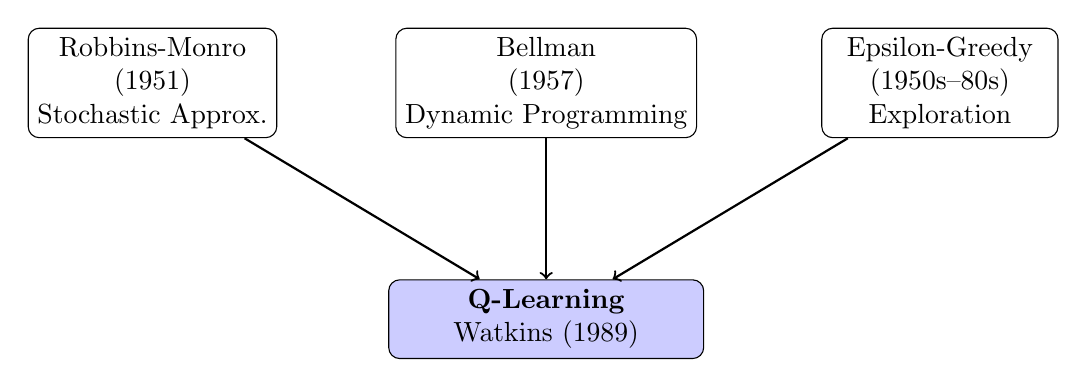
\begin{tikzpicture}[
    box/.style={rectangle, draw, rounded corners, minimum width=3cm, minimum height=1cm, align=center},
    arrow/.style={->, thick}
]
\node[box] (rm) at (0,3) {Robbins-Monro\\(1951)\\Stochastic Approx.};
\node[box] (bell) at (5,3) {Bellman\\(1957)\\Dynamic Programming};
\node[box] (eg) at (10,3) {Epsilon-Greedy\\(1950s--80s)\\Exploration};

\node[box, fill=blue!20, minimum width=4cm] (ql) at (5,0) {\textbf{Q-Learning}\\Watkins (1989)};

\draw[arrow] (rm) -- (ql);
\draw[arrow] (bell) -- (ql);
\draw[arrow] (eg) -- (ql);
\end{tikzpicture}
\end{center}

\vspace{0.5cm}
\textbf{Q-Learning = Robbins-Monro + Bellman + Epsilon-Greedy}

\vspace{0.3cm}
A beautiful synthesis of ideas spanning 40 years of mathematics, operations research, and computer science.
\end{frame}

\begin{frame}{References}
\footnotesize
\begin{itemize}
    \item Robbins, H. \& Monro, S. (1951). A stochastic approximation method. \textit{Annals of Mathematical Statistics}.
    \item Bellman, R. (1957). \textit{Dynamic Programming}. Princeton University Press.
    \item Watkins, C. (1989). \textit{Learning from Delayed Rewards}. PhD thesis, Cambridge.
    \item Watkins, C. \& Dayan, P. (1992). Q-learning. \textit{Machine Learning}.
    \item Sutton, R. \& Barto, A. (2018). \textit{Reinforcement Learning: An Introduction}. 2nd ed.
    \item Mnih, V. et al. (2015). Human-level control through deep reinforcement learning. \textit{Nature}.
\end{itemize}
\end{frame}

\end{document}
